\chapter{Schema bazy i partycjonowanie}
	\section{Tabela partycjonowana}
	
	\section{Widok i tabela tymczasowa}
	
Istnieją dwie formy dostępu do bazy danych w oparciu o tymczasową lub ograniczoną wersję danych. Są to widoki oraz tabele tymczasowe.
Widok nie zmienia w żaden sposób danych źródłowych, lecz każdorazowo wykonuje zapytanie typu SELECT do tabel źródłowych. Zaletą jest oszczędność miejsca na dysku, dane nie są duplikowane, podstawową wadą takiego rozwiązania jest czas wykonania zapytania do widoku - szczególnie w przypadku skomplikowanych konwersji.
Widok tworzymy poleceniem:
\begin{lstlisting}
CREATE VIEW nazwa AS SELECT * FROM tabela;
\end{lstlisting} 
Szczególną formą jest widok zmaterialiowany - dane wynikowe są przechowywane w gotowej postaci, lecz w każdej chwili można je zaktualizować przy pomocy predefiniowanego zapytania. Służą do tego następujące polecenia:
\begin{lstlisting}
CREATE MATERIALIZED VIEW widok_m AS SELECT x FROM y;
REFRESH MATERIALIZED VIEW widok_m;
\end{lstlisting}
Innym rozwiązaniem, szybszym i wydajniejszym od widoku jest tabela tymczasowa. Tworzona jest ona tylko na czas trwania danej sesji w psql. Taka forma jest szczególnie wygodna wtedy gdy dane które będą przechowywane w tej tabeli, mają służyć do zagregowania, czy innej analityki, a następnie będą usuwane.
\begin{lstlisting}
CREATE TEMPORARY TABLE nazwa AS ... ON COMMIT operacja;
\end{lstlisting}
gdzie wartość parametru operacja to - PRESERVE ROWS, DELETE ROWS lub DROP.
	
	\section{Schema bazy danych}

Schemat bazy danych to nazwana kolekcja elementów bazy danych. Może zawierać tabele, widoki, indeksy, sekwencje, typy danych, operatory i funkcje. Najbliższym odpowiednikiem w systemie operacyjnym jest katalog. Jednak w przypadku schematu bazy danych zagnieżdżanie jest niemożliwe. Jako główną przyczynę wykorzystania schematu bazy danych możemy wymienić konieczność rozdzielenia użytkowników i/lub aplikacji, tak, aby nazwy tworzonych obiektów (np. tabele tymczasowe), nie kolidowały ze sobą.

\begin{figure}[!ht]
	\centering
	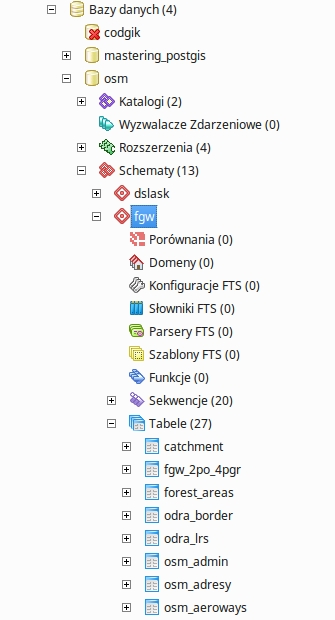
\includegraphics[width=6cm]{pgadmin_schemy}
	\caption{pgAdmin - zawartość przykładowego schematu}
\end{figure}
W analogii do tworzenia tabeli schemat bazy danych tworzymy wywołaniem \colorbox{code-gray}{CREATE SCHEMA nazwa;}
Aby przenieść istniejącą tabelę do wybranej schemy wykorzystujemy słowo kluczowe ALTER.
\begin{lstlisting}
ALTER TABLE nazwa\_tabeli SET SCHEMA nazwa\_schemy;
\end{lstlisting}

Należy pamiętać że domyślnie PostgreSQL wyszukuje tabele wyłącznie w schemacie \textit{public}. Jeśli chcemy ułatwić sobie życie, skorzystajmy z następującej zmiennej środowiskowej.
\begin{lstlisting}
SET search_path = nazwa_schemy, public;
\end{lstlisting}
Dla narzędzi typu pgAdmin nie ma konieczności ustawiania takich zmiennych, dba o to oprogramowanie.
